    We define and characterize the robot multistable joint in the following order. First, by describing the working principle of a simple bistable mechanism that will then be used in series to create a multistable joint. The multistable joint will create the main structure of the robot's leg. Finally, the sequences principle and description between the joint's stable states will be derived.

    \section{Bistable joint design}
    \label{sec:bistable}
    \begin{figure}
        \centering
        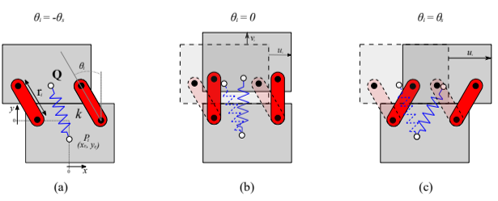
\includegraphics[width=1.0\textwidth]{images/basics_building_blocks.png}
        \caption{Schematics showing our basic building structure. It is composed of one bottom block, considered as fixed, and a top block that we can displace. The two blocks are linked together using arms of length $r_i$ and anchor distance $\delta$ represented in red. A linear spring is also linking the two blocks together, with an anchor on the bottom block that can be changed. This structure is therefore pulling the top block toward the bottom block and depending on the spring anchor location, it will create two stable resting states. If the top block is on the left side, we call this \textit{state 0}, on the right we call this \textit{state 1}}
        \label{fig:joint_basics}
    \end{figure}
    We first start with the basic structure of our joint, which consists of two rectangular blocks, one on top of the other as shown in Figure \ref{fig:joint_basics}. Those two blocks are linked together using a parallelogram linkage to constrain the displacement of the top block relative to the bottom one. We consider the bottom block to be connected to the frame, therefore we can have a horizontal input displacement on the top block. The horizontal displacement of the top block is constrained by the length of the arms ($r_i$) and the distance between arm's anchor point to the side of the block ($\delta$). We define $\theta_i$ as the angle between the $y$ (vertical) axis and the longitudinal axis of the arm, it is positive when the block is positioned on the right. $\theta_i$ is bounded by two angles: $-\theta_s$ and $+\theta_s$ obtained using Equation \ref{eq:theta_s}. Once $\theta_s$ known, the total horizontal stroke ($h_{tot}$) for the top block can be computed using Equation \ref{eq:max_dist}. The vertical displacement ($y$) of the block can be computed using $\theta_i$ and Equation \ref{eq:y_block}.
    
    \begin{equation}
        \theta_s = cos^{-1}\left(\frac{2\delta}{r_i}\right)
        \label{eq:theta_s}
    \end{equation}
    \begin{equation}
        h_{tot} = 2 sin(\theta_s) r_i
        \label{eq:max_dist}
    \end{equation}
    \begin{equation}
        v_i = cos(\theta_i) r_i
        \label{eq:y_block}
    \end{equation}
    
    A preloaded tensile spring is attached between the two blocks with two anchors, $Q$ and $P$. $Q$ is positioned horizontally in the middle of the top block and vertically at a distance $\delta$ from top block side. $P$ anchor is positioned in the bottom block at the position $(x_P, y_P)$.
    The spring is considered linear with a stiffness $k$ and a rest length $l_0$. The potential energy stored in the spring can be described using Equation \ref{eq:potential_single} \cite{mo_main_paper}. From this equation, a local maximum can be determined using Equation \ref{eq:snap_angle}. This local maximum is at the angle where the block would be at an unstable equilibrium point. If the angle increase beyond $\theta_{snap}$, the top block would snap and rest on the $\theta_s$ position. On the other side, if the angle is below $\theta_{snap}$, the top block would snap and rest on the $-\theta_s$ position.\\
    
   Caused by the potential energy stored in the spring, the block can have one or two resting states. Figure \ref{fig:energy} is an example of different configuration for the bistable joint where the energy is stored differently along with the angle value. Each line corresponds to the energy stored in the spring depending on the angle. Each line represents a different anchor point. The blue line is where the anchor position is centered ($0$, $0$) and produce the expected two stable states in a symmetric shape. The orange line is where the anchor point is displaced to the left ($-0.25$, $0$), the local maximum is more to the right. This means the snapping would occur at a different position than for a centered anchor. The extreme case is the green line where the anchor position is further away ($-1$, $0$) and it shows that there is now only one local minimum while for the two other lines, two local minima exist. This implies there is now only one stable state for the system. To simplify the description, \textit{state 0} defines the position of the top block being on the left with an angle of $-\theta_s$ and \textit{state 1}  defines the position of the top block being on the right with an angle of $\theta_s$. This basic structure will help the creation of a multistable system that will be used to create the robot's legs. 
    

    \begin{equation}
        \epsilon = \frac{k}{2}\left(\sqrt{(r_i sin\theta_i - x_P)^2 + (r_i cos\theta_i - y_P)^2} - l_0^2\right)    
        \label{eq:potential_single}
    \end{equation}
    \begin{equation}
        \theta_{snap} = tan^{-1}\left(\frac{x_P}{y_P}\right)    
        \label{eq:snap_angle}
    \end{equation}
    
    \begin{figure}
        \centering
        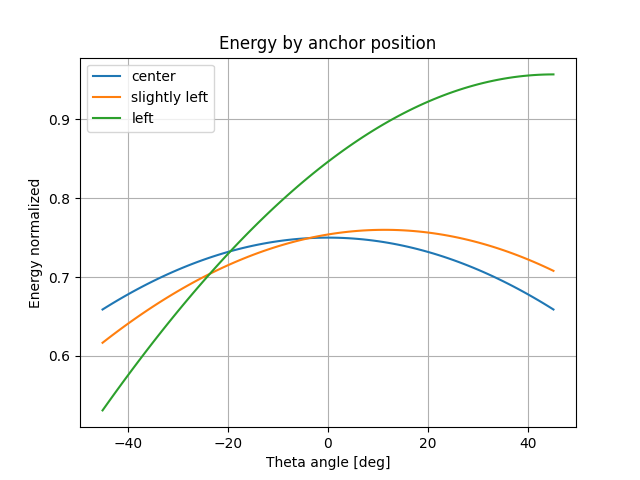
\includegraphics[width=0.7\textwidth]{images/energy.png}
        \caption{This figure shows the amount of energy stored inside the spring. The horizontal axis represents the angle between the arms and the vertical axis, the vertical axis is a normalized quantity of energy stored and there are three different cases, where the anchor is at a different position. In the center, slightly to the left, or to the extreme left. This shows how the snapping position displaces from center to the right. The green case shows that for a specific condition it is possible to find only one stable state instead of two. }
        \label{fig:energy}
    \end{figure}
    
    
    
    \section{Multistable joint design}\label{sec:mutistable}
        The multistable joint is an evolution of the bistable joint by putting two bistable joints in series. Figure \ref{fig:joint_multistable} shows how two bistable joints are stacked together. The multistable joint consists of three blocks. The bottom block is anchored to the ground, the middle block is linked to the bottom one with two arms of length $r_1$. The associated spring from the bottom bistable joint has an anchor at position $(x_{P_1}, y_{P_1})$. Finally, the top block is linked to the middle block in a similar way. Arms between the middle and the top block have a length $r_2$. The second bistable spring has an anchor point at position $(x_{P_2}, y_{P_2})$. 
        Both bistable joint has their own $theta_{i_1}$, $theta_{i_2}$ and horizontal maximum strokes.\\
        
        \begin{figure}
        \centering
        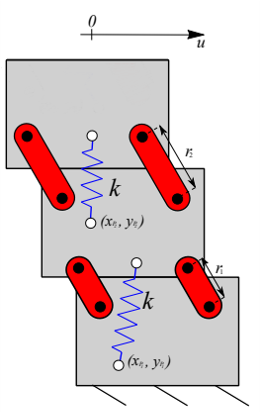
\includegraphics[width=0.40\textwidth]{images/multistable.png}
        \caption{Schematic of a multistable joint build with two bistable joint assembled in serie. Parameters such as arms lengths, springs anchor position define the number of stable states we may have. We can define 4 states: $00$ when $\theta_{i_1} = -\theta_{s_1}$ and $\theta_{i_2} = -\theta_{s_2}$; $01$ when $\theta_{i_1} = -\theta_{s_1}$ and $\theta_{i_2} = +\theta_{s_2}$; $10$ when $\theta_{i_1} = +\theta_{s_1}$ and $\theta_{i_2} = -\theta_{s_2}$; $11$ when $\theta_{i_1} = +\theta_{s_1}$ and $\theta_{i_2} = +\theta_{s_2}$}
        \label{fig:joint_multistable}
        \end{figure}
        
        When building multiple bistable joints together, the total potential energy stored in the mechanism is described by Equation \ref{eq:potential}. In this equation, $\theta_i$ describe the angle between the $i$-th pair of levers with the vertical axis, $r_i$ describe the length of the $i$-th arms, $x_{P_i}$ and $y_{P_i}$ describe the anchor position of the $i$-th spring. As explained in Dr. Zanaty's paper \cite{mo_main_paper}, the equation determine different anchor position to create multiple stable positions and more importantly, the snapping point determined by the equation can vary from the bottom bistable joint to the top bistable joint. This can create situations where the bottom block would snap before the bottom block for example. Regarding the number of stable positions, Equation \ref{eq:potential} give in the case of two bistable joints in series four potential stable positions. Those different positions occur at each local minima. This joint is quadristable.

        \begin{equation}
            \epsilon_{tot} = \frac{k}{2} \sum_{i=1}^{N}\left(\sqrt{(r_i sin \theta_i - x_{P_i})^2 + (r_i cos \theta_i - y_{P_i})^2} \right) - l_0^2
            \label{eq:potential}
        \end{equation}
        
        As previously defined in the bistable joint, stable positions from the multistable joint will be defined as \textit{states}. Each bistable block can be in either in \textit{state 0} or \textit{state 1}. As the multistable joint consists of two bistable mechanisms, two numbers will be used to describe the state of the multistable joint. The first number will represent the state of the bottom bistable joint while the second number will represent the state of the top bistable joint. Therefore we have four possible states described as follow:\\
        \begin{itemize}
            \item $00$ when $\theta_{i_1} = -\theta_{s_1}$ and $\theta_{i_2} = -\theta_{s_2}$; (Both blocks on the left)
            \item $10$ when $\theta_{i_1} = +\theta_{s_1}$ and $\theta_{i_2} = -\theta_{s_2}$; (Middle block on the right, Top block on the left)
            \item $01$ when $\theta_{i_1} = -\theta_{s_1}$ and $\theta_{i_2} = +\theta_{s_2}$; (Middle block on the left, Top block on the right)
            \item $11$ when $\theta_{i_1} = +\theta_{s_1}$ and $\theta_{i_2} = +\theta_{s_2}$; (Both blocks on the right)
        \end{itemize}
        
        The order of states occurrence will determine the type of sequences as we will see in Section \ref{sec:sequences}. The multistable joint is always actuated from the top block. We define the origin by the \textit{state 00} resting point.
        
    \section{Multistable joint sequences}\label{sec:sequences}
        The multistable joint defined previously has different possible states (\textit{00; 01; 10; 11}), those states may be reached when a specific scenario is triggered. Equation \ref{eq:potential} shows the potential energy stored in the system for a combination of angles. As seen previously, the anchor position of a spring will determine the number of stable states, but also the angle at which the snap occurs. Therefore if two springs have different anchor points, and a displacement of the top block is applied, there is a situation where the top block would move with the actuation, but the middle block would stay in place. There is also a situation with different anchor positions where the middle block and the top block would move together with the actuation, resulting in the top block having no displacement relative to the middle block. This difference is defined as having different sequences.\\
        The actuation will always do a cycle, starting from the \textit{state 00}, touching the \textit{state 11} and going back to the \textit{state 00}. This cycle is defined as a sequence. A sequence is a path that starts and end at \textit{state 00} and reach at a certain point the \textit{state 11}. Those sequences can be represented as a final state machine that contains four states. Figure \ref{fig:sequences} shows the different sequences that our multistable joint will be able to reach \cite{mo_main_paper}. As recall, the first state's number represents the middle block's position while the second number represents top block's position. Left position ($-\theta_s$) is represented by a $0$ and right position ($+\theta_s$) is expressed by a $1$. As the path along the cycle may not be symmetrical, it is important to dissociate the path followed in forward motion from the path followed in backward motion. Figure \ref{fig:sequences} shows the ten possible sequences a multistable joint can perform in a cycle. The green arrows represent the forward path while the red arrows represent the backward path. \\
        
        
        \begin{figure}
            \begin{tabular}{cccc}
                \subfloat[Sequence A]{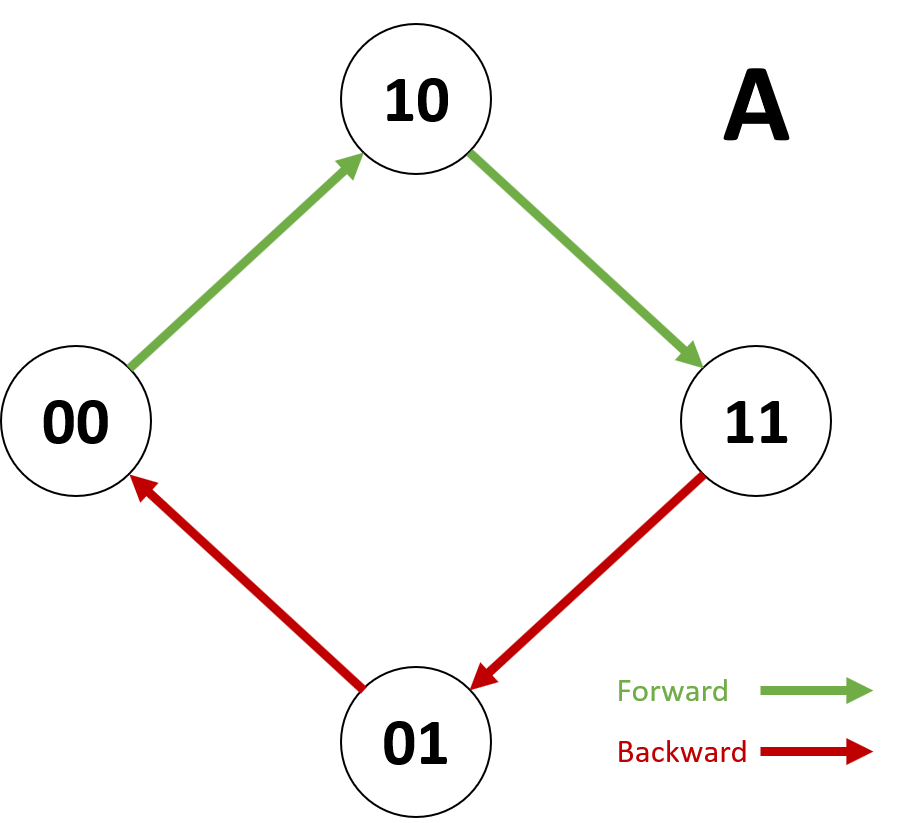
\includegraphics[width = 1.5in]{images/S_A.png}} &
                \subfloat[Sequence B]{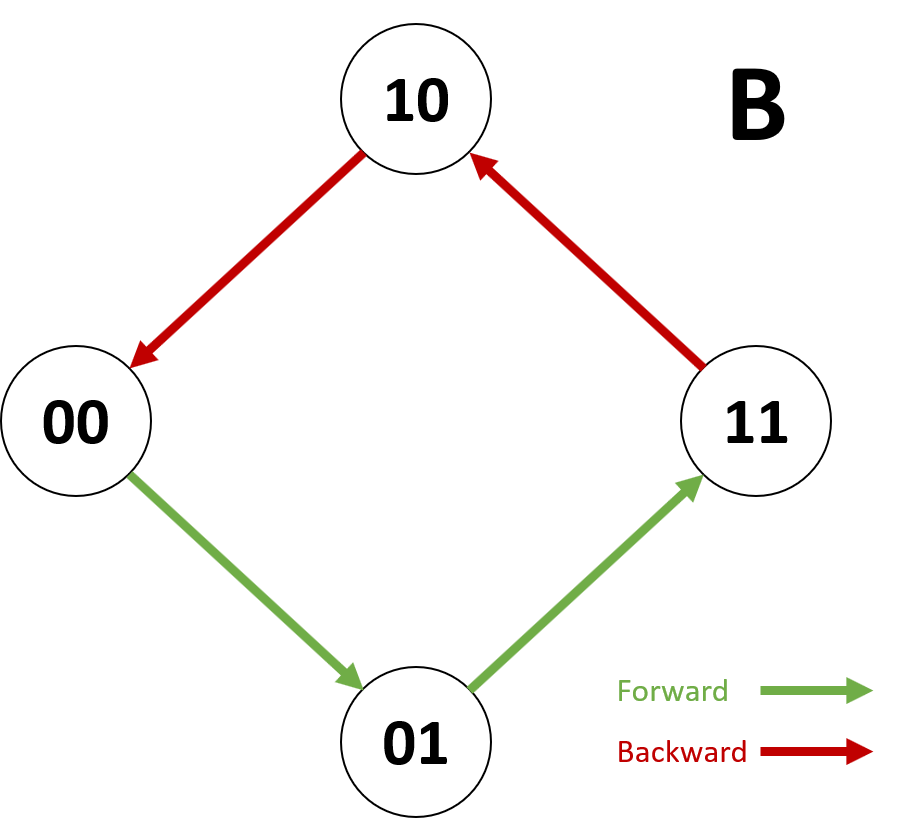
\includegraphics[width = 1.5in]{images/S_B.png}} &
                \subfloat[Sequence C]{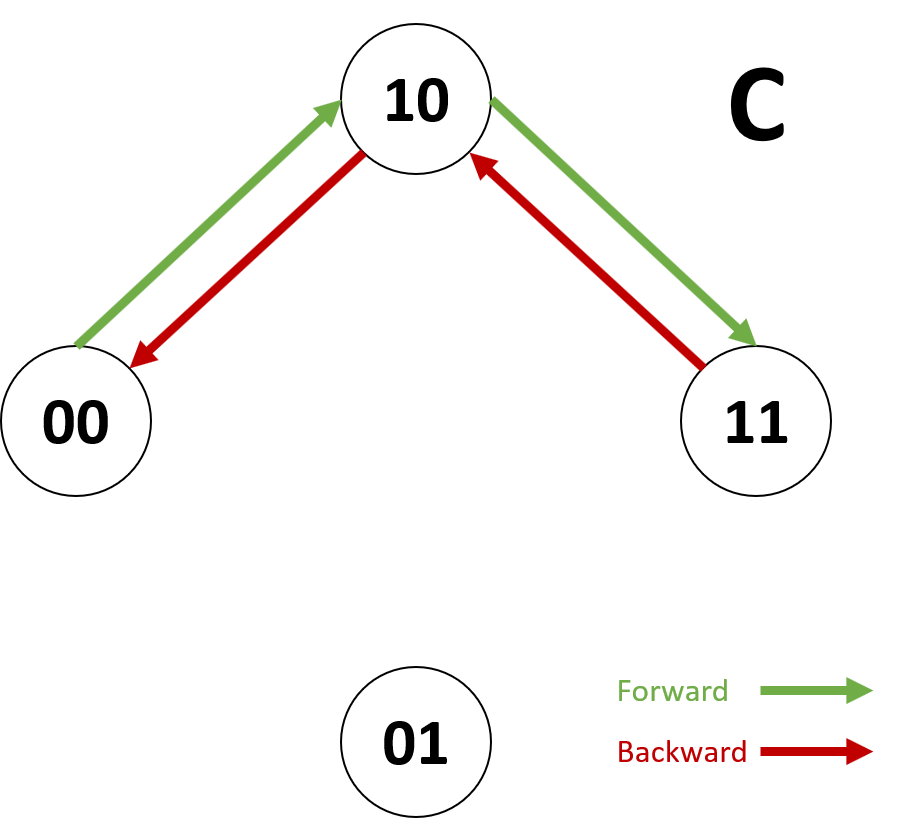
\includegraphics[width = 1.5in]{images/S_C.png}} &
                \subfloat[Sequence D]{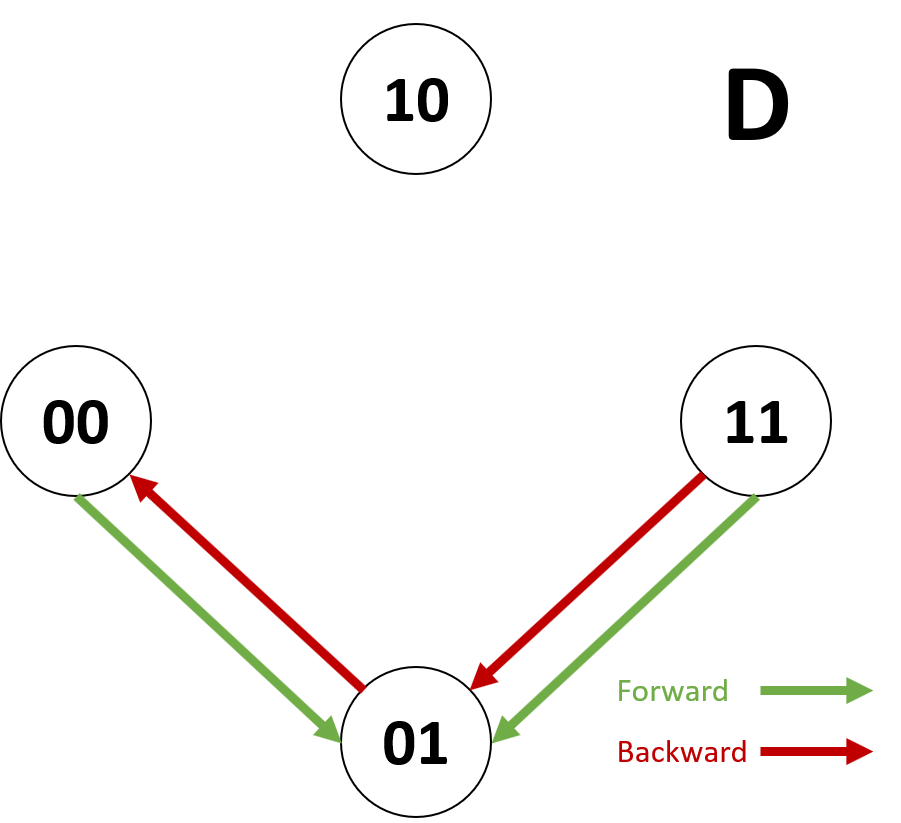
\includegraphics[width = 1.5in]{images/S_D.png}} \\
                \subfloat[Sequence E]{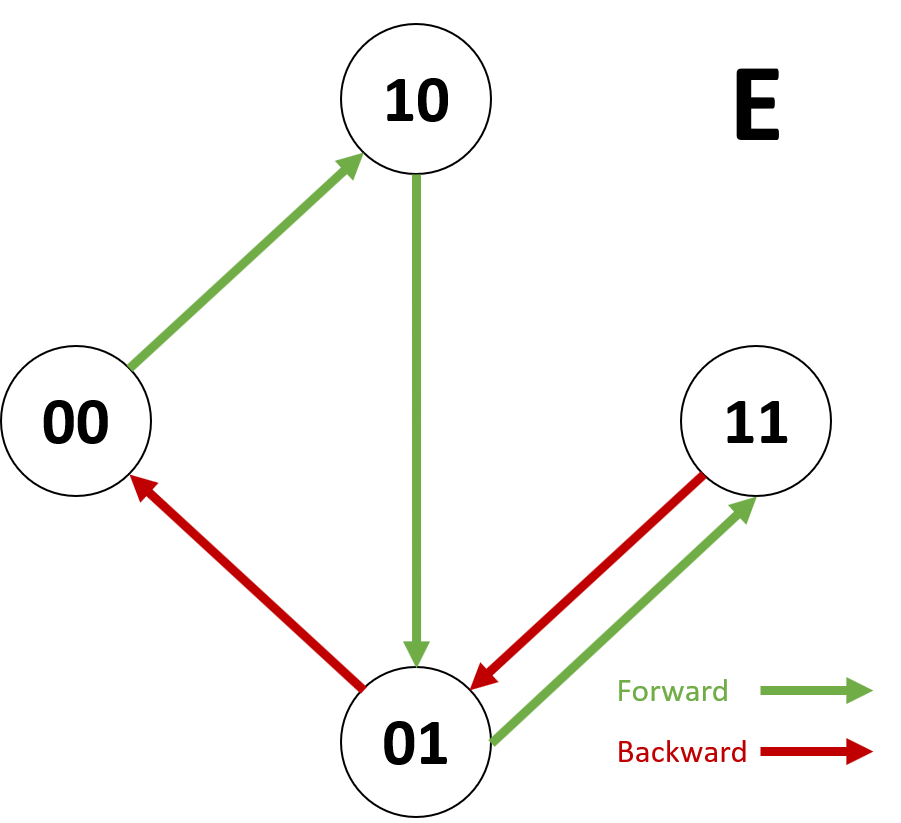
\includegraphics[width = 1.5in]{images/S_E.png}} &
                \subfloat[Sequence F]{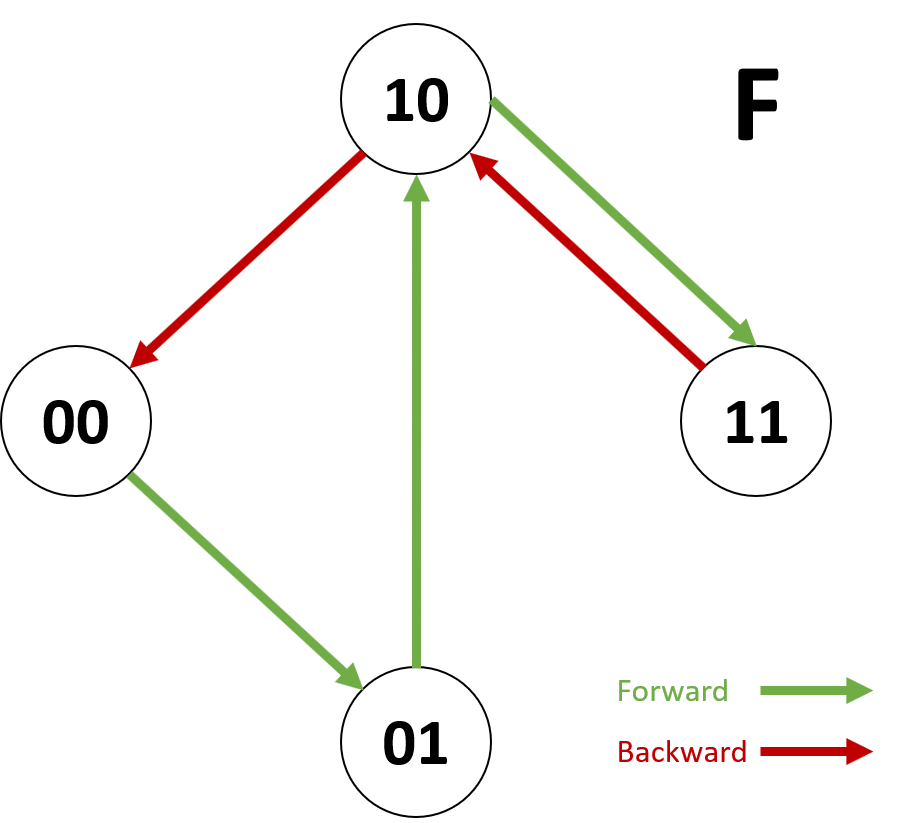
\includegraphics[width = 1.5in]{images/S_F.png}} &
                \subfloat[Sequence G]{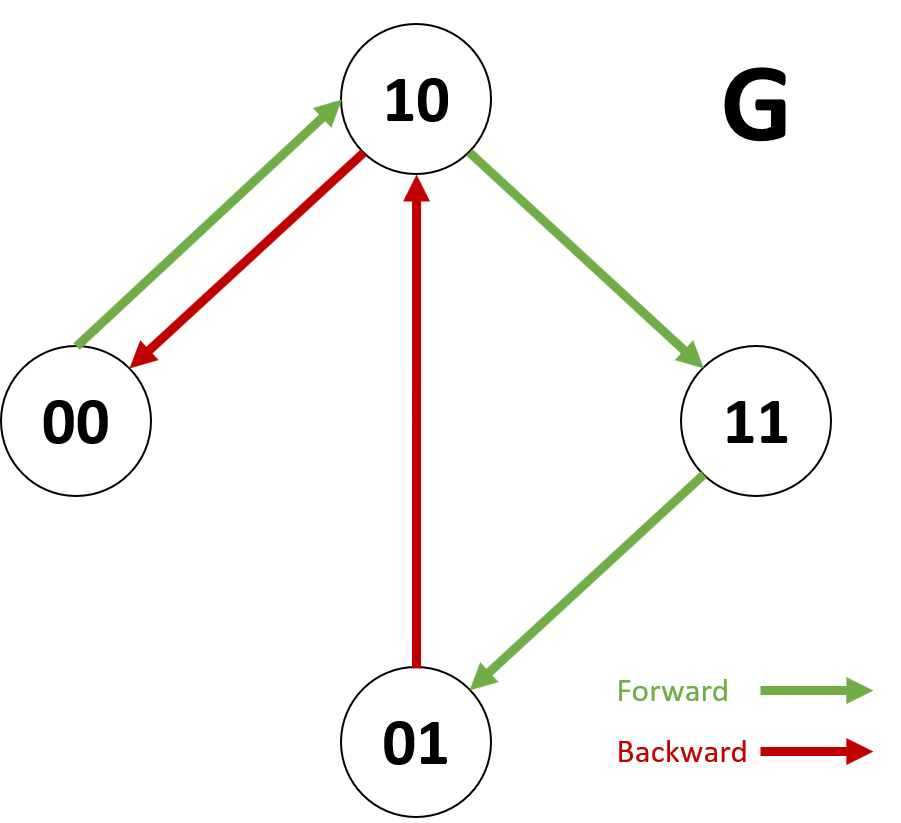
\includegraphics[width = 1.5in]{images/S_G.png}} &
                \subfloat[Sequence H]{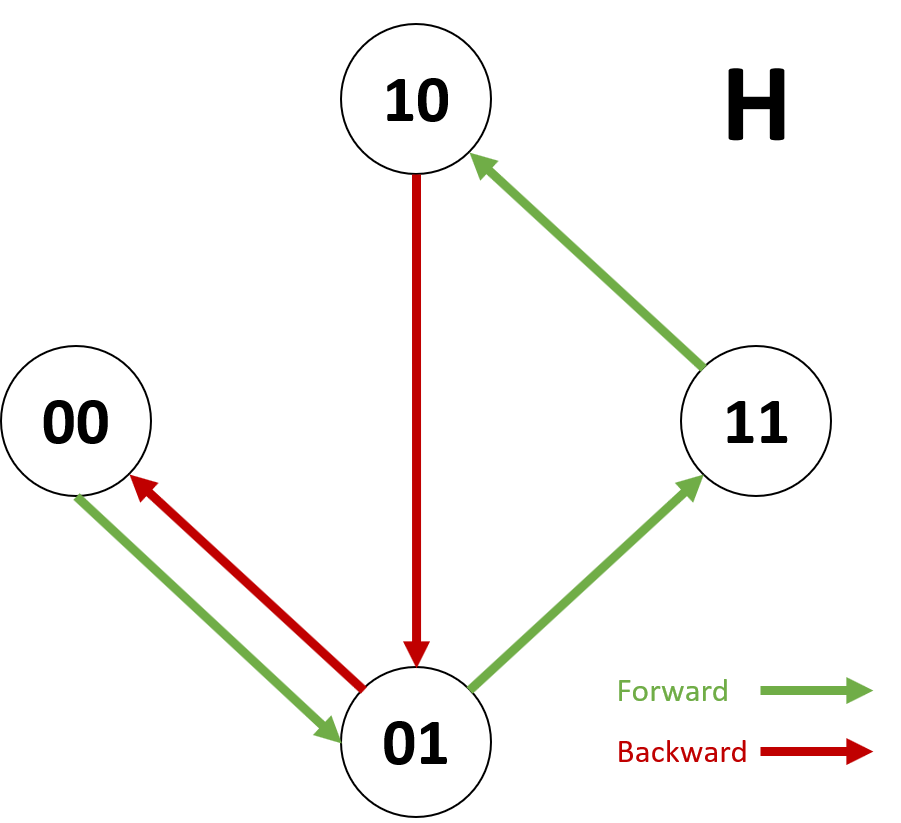
\includegraphics[width = 1.5in]{images/S_H.png}} \\
                & 
                \subfloat[Sequence I]{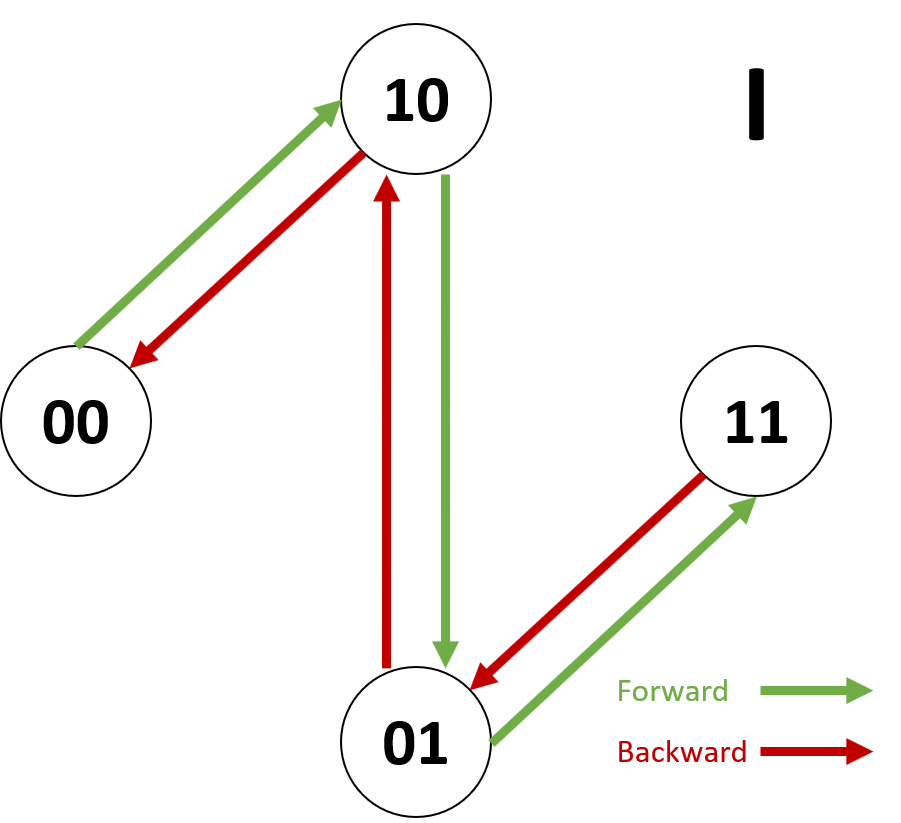
\includegraphics[width = 1.5in]{images/S_I.png}} &
                \subfloat[Sequence J]{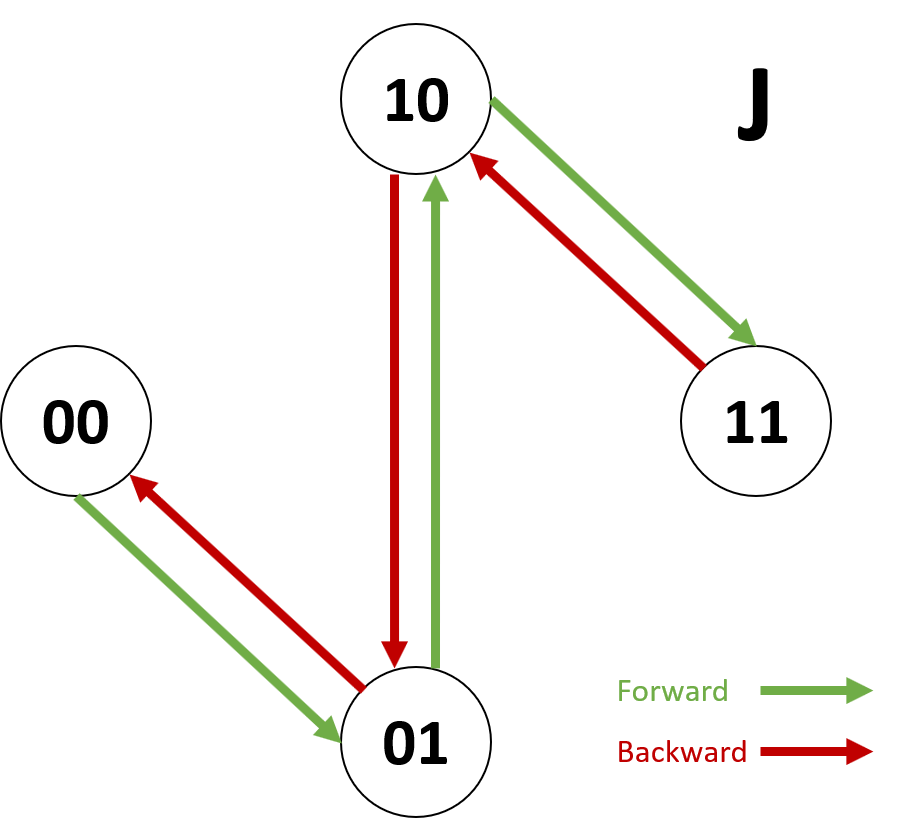
\includegraphics[width = 1.5in]{images/S_J.png}} &

            \end{tabular}
            \caption{Final state representation of the different types of sequences allowed in the quadristable joint. There are four different states, the first number representing the middle block's position, the second number representing the top block's position. When block's position is on the left, the state is $0$, $1$ block's position is on the right. Each sequence start and end at \textit{state 00} and need to reach \textit{state 11}. The path used in forward or backward motion may differ.}
            \label{fig:sequences}
        \end{figure}
        
        There are ten possible sequences shown in Figure \ref{fig:sequences} and there are two main categories. Sequences A-D are the four basic sequences while sequences E-J uses \textit{avalanche} principle to swap blocks position in the middle of a cycle \cite{mo_main_paper}. 

        
    